\documentclass{article}
\usepackage{booktabs}
\usepackage{amsmath}
\usepackage{amssymb}
\usepackage[noend]{algorithmic}
\usepackage[nothing]{algorithm}
\usepackage{tikz}
\usepackage{latexsym}
\usepackage{float}
\providecommand{\e}[1]{\ensuremath{\times 10^{#1}}}
\renewcommand{\thealgorithm}{}
\usetikzlibrary{arrows}
\title{CS 522: Data Structures and Algorithms II \\ Homework 1}
\author{Dustin Ingram}
\begin{document}
\maketitle
\begin{enumerate}
    \item \textbf{Solution:}
    If both \textsc{Increment} and \textsc{Decrement} operations were included
    in the $k$-bit counter, an amortized analysis of the cost of $n$ operations
    would cost as much as $\Theta(nk)$ time because we would no longer be able
    to consider each operation as a consecutive \textsc{Increment}, but rather
    as any combination of \textsc{Increment}s and \textsc{Decrement}s. Thus, in
    a worse-case scenario, it would be possible to alternate $n$ times between
    two operations which cost $O(k)$ each, resulting in a total cost of
    $\Theta(nk)$.

    \item \textbf{Solution:}
    To show that the amortized cost of \textsc{Table-Delete} under this strategy
    is bounded above by a constant, we will consider two cases. We will use the
    potential function:

    $$ \Phi(T) = | 2\cdot T.num - T.size | $$

    The first case is the one in which the table does not contract, and thus
    $num_{i} = num_{i-1}-1$, $size_{i} = size_{i-1}$, and $c_{i} = 1$:

    \begin{eqnarray*}
        \hat{c_{i}} &=& c_{i} + \Phi_{i} - \Phi_{i-1} \\
        \hat{c_{i}} &=& 1 + |2\cdot num_{i} - size_{i}| - | 2\cdot num_{i-1} - size_{i-1} | \\
        \hat{c_{i}} &=& 1 + |2\cdot(num_{i-1} - 1) - size_{i-1}| - | 2\cdot num_{i-1} - size_{i-1} | \\
        \hat{c_{i}} &=& 1 + |-2| \\
        \hat{c_{i}} &=& 3 \\
    \end{eqnarray*}

    The second case is the one in which the table does contract, and thus
    $size_{i} = \frac{2}{3}size_{i-1}$, $num_{i-1} = \frac{1}{3}size_{i-1}$, and
    $c_{i} = num_{i} + 1$:

    \begin{eqnarray*}
        \hat{c_{i}} &=& c_{i} + \Phi_{i} - \Phi_{i-1} \\
        \hat{c_{i}} &=& (num_{i} +1) + |2\cdot num_{i} - size_{i}| - | 2\cdot num_{i-1} - size_{i-1} | \\
        \hat{c_{i}} &=& ((num_{i-1} - 1) + 1) + |2\cdot(num_{i-1} - 1) - \frac{2}{3}size_{i-1}| - | 2\cdot num_{i-1} - size_{i-1} | \\
        \hat{c_{i}} &=& (num_{i-1}) + |-2 + \frac{1}{3}size_{i-1}| \\
        \hat{c_{i}} &=& 2 \\
    \end{eqnarray*}

    Thus we see that the amortized cost of \textsc{Table-Delete} is at most 3
    and is thus bounded.

    \item \textbf{Solution:}
    One can use the following sequence to produce a Fibonacci heap that is only
    a linear chain of $n$ nodes. Since we start at the base case (where the heap
    is empty) and create a chain of a single node, followed by a chain of two
    nodes from a chain of one node, and then a chain of three nodes from a chain
    of two nodes, we can repeat the process $n$ times to produce a chain of
    total length $n$.

    \textsc{Fib-Heap-Insert}(H, $m$):
    \begin{figure}[H]
    \centering
    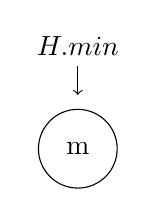
\begin{tikzpicture}[
      level 1/.style={sibling distance=48mm, level distance=10mm},
      level 2/.style={sibling distance=16mm, level distance=10mm},
      level 3/.style={sibling distance=8mm, level distance=10mm},
    ]
    \node [circle,draw, minimum size=1cm] (1){m};
    \node [above of=1, yshift=.3cm] (min) {$H.min$};
    \path [draw, ->, shorten >=5pt] (min)--(1.north);
    \end{tikzpicture}
    \end{figure}

    \textsc{Fib-Heap-Insert}(H, $m-1$):
    \begin{figure}[H]
    \centering
    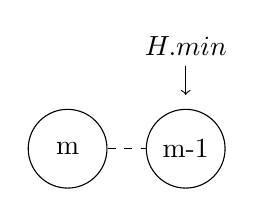
\begin{tikzpicture}[
      level 1/.style={sibling distance=100mm, level distance=10mm},
      level 2/.style={sibling distance=16mm, level distance=10mm},
      level 3/.style={sibling distance=100mm, level distance=10mm},
      node distance=1.5cm
    ]
    \node [circle,draw, minimum size=1cm] (1){m};
    \node [circle,draw, minimum size=1cm, right of=1] (2){m-1};
    \path [draw, dashed] (1)--(2);
    \node [above of=2, yshift=-.2cm] (min) {$H.min$};
    \path [draw, ->, shorten >=5pt] (min)--(2.north);
    \end{tikzpicture}
    \end{figure}

    \textsc{Fib-Heap-Insert}(H, $m-2$):
    \begin{figure}[H]
    \centering
    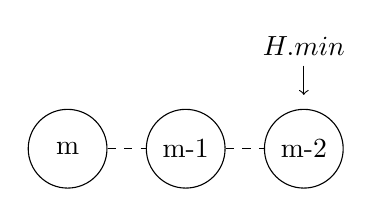
\begin{tikzpicture}[
      level 1/.style={sibling distance=48mm, level distance=10mm},
      level 2/.style={sibling distance=16mm, level distance=10mm},
      level 3/.style={sibling distance=8mm, level distance=10mm},
      node distance=1.5cm
    ]
    \node [circle,draw, minimum size=1cm] (1){m};
    \node [circle,draw, minimum size=1cm, right of=1] (2){m-1};
    \node [circle,draw, minimum size=1cm, right of=2] (3){m-2};
    \path [draw, dashed] (1)--(2);
    \path [draw, dashed] (2)--(3);
    \node [above of=3, yshift=-.2cm] (min) {$H.min$};
    \path [draw, ->, shorten >=5pt] (min)--(3.north);
    \end{tikzpicture}
    \end{figure}

    \textsc{Fib-Heap-Extract-Min}(H):
    \begin{figure}[H]
    \centering
    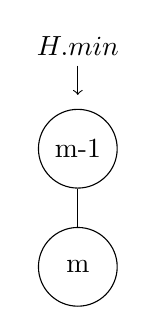
\begin{tikzpicture}[
      level 1/.style={sibling distance=48mm, level distance=10mm},
      level 2/.style={sibling distance=16mm, level distance=10mm},
      level 3/.style={sibling distance=8mm, level distance=10mm},
      node distance=1.5cm
    ]
    \node [circle,draw, minimum size=1cm] (1){m-1}
     child {node [circle,draw, minimum size=1cm, below of=1] (3){m}};
    \node [above of=1, yshift=-.2cm] (min) {$H.min$};
    \path [draw, ->, shorten >=5pt] (min)--(1.north);
    \end{tikzpicture}
    \end{figure}

    \textsc{Fib-Heap-Insert}(H, $m-3$):
    \begin{figure}[H]
    \centering
    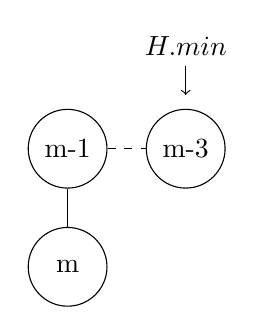
\begin{tikzpicture}[
      level 1/.style={sibling distance=48mm, level distance=10mm},
      level 2/.style={sibling distance=16mm, level distance=10mm},
      level 3/.style={sibling distance=8mm, level distance=10mm},
      node distance=1.5cm
    ]
    \node [circle,draw, minimum size=1cm] (1){m-1}
     child {node [circle,draw, minimum size=1cm, below of=1] (2){m}};
    \node [circle, draw, minimum size=1cm, right of=1] (4){m-3};
    \path [draw, dashed] (1)--(4);
    \node [above of=4, yshift=-.2cm] (min) {$H.min$};
    \path [draw, ->, shorten >=5pt] (min)--(4.north);
    \end{tikzpicture}
    \end{figure}

    \textsc{Fib-Heap-Insert}(H, $m-4$):
    \begin{figure}[H]
    \centering
    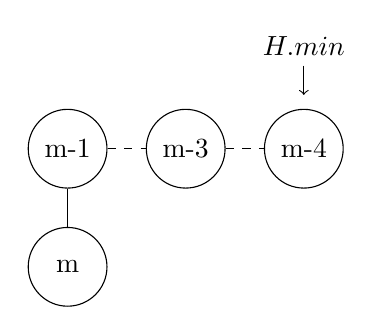
\begin{tikzpicture}[
      level 1/.style={sibling distance=48mm, level distance=10mm},
      level 2/.style={sibling distance=16mm, level distance=10mm},
      level 3/.style={sibling distance=8mm, level distance=10mm},
      node distance=1.5cm
    ]
    \node [circle,draw, minimum size=1cm] (1){m-1}
     child {node [circle,draw, minimum size=1cm, below of=1] (2){m}};
    \node [circle, draw, minimum size=1cm, right of=1] (4){m-3};
    \node [circle, draw, minimum size=1cm, right of=4] (5){m-4};
    \path [draw, dashed] (1)--(4);
    \path [draw, dashed] (4)--(5);
    \node [above of=5, yshift=-.2cm] (min) {$H.min$};
    \path [draw, ->, shorten >=5pt] (min)--(5.north);
    \end{tikzpicture}
    \end{figure}

    \textsc{Fib-Heap-Insert}(H, $m-5$):
    \begin{figure}[H]
    \centering
    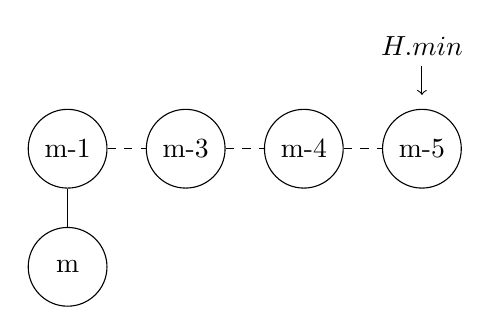
\begin{tikzpicture}[
      level 1/.style={sibling distance=48mm, level distance=10mm},
      level 2/.style={sibling distance=16mm, level distance=10mm},
      level 3/.style={sibling distance=8mm, level distance=10mm},
      node distance=1.5cm
    ]
    \node [circle,draw, minimum size=1cm] (1){m-1}
     child {node [circle,draw, minimum size=1cm, below of=1] (2){m}};
    \node [circle, draw, minimum size=1cm, right of=1] (4){m-3};
    \node [circle, draw, minimum size=1cm, right of=4] (5){m-4};
    \node [circle, draw, minimum size=1cm, right of=5] (6){m-5};
    \path [draw, dashed] (1)--(4);
    \path [draw, dashed] (4)--(5);
    \path [draw, dashed] (5)--(6);
    \node [above of=6, yshift=-.2cm] (min) {$H.min$};
    \path [draw, ->, shorten >=5pt] (min)--(6.north);
    \end{tikzpicture}
    \end{figure}

    \textsc{Fib-Heap-Extract-Min}(H):
    \begin{figure}[H]
    \centering
    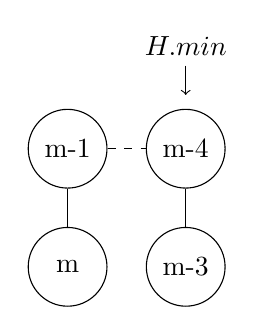
\begin{tikzpicture}[
      level 1/.style={sibling distance=48mm, level distance=10mm},
      level 2/.style={sibling distance=16mm, level distance=10mm},
      level 3/.style={sibling distance=8mm, level distance=10mm},
      node distance=1.5cm
    ]
    \node [circle,draw, minimum size=1cm] (1){m-1}
     child {node [circle,draw, minimum size=1cm, below of=1] (2){m}};
    \node [circle, draw, minimum size=1cm, right of=1] (4){m-4}
     child {node [circle, draw, minimum size=1cm, below of=4] (5){m-3}};
    \path [draw, dashed] (1)--(4);
    \path [draw, dashed] (4)--(5);
    \node [above of=4, yshift=-.2cm] (min) {$H.min$};
    \path [draw, ->, shorten >=5pt] (min)--(4.north);
    \end{tikzpicture}
    \end{figure}

    \textsc{Fib-Heap-Delete(H, $m-3$)}:
    \begin{figure}[H]
    \centering
    \begin{tikzpicture}[
      level 1/.style={sibling distance=48mm, level distance=10mm},
      level 2/.style={sibling distance=16mm, level distance=10mm},
      level 3/.style={sibling distance=8mm, level distance=10mm},
      node distance=1.5cm
    ]
    \node [circle, draw, minimum size=1cm, right of=1] (4){m-4}
     child {node [circle, draw, minimum size=1cm, below of=4] (5){m-1}
      child {node [circle,draw, minimum size=1cm, below of=5] (2){m}}};
    \node [above of=4, yshift=-.2cm] (min) {$H.min$};
    \path [draw, ->, shorten >=5pt] (min)--(4.north);
    \end{tikzpicture}
    \end{figure}

    \item \textbf{Solution:}

    \item \textbf{Solution:}

    \item \textbf{Solution:}

    \item \textbf{Solution:}

    \item \textbf{Solution:}
\end{enumerate}
\end{document}
